\documentclass[a4paper,12pt,oneside,English]{article}
\usepackage[a4paper,top=1.5cm,bottom=1.5cm,left=1cm,right=1cm]{geometry}
\usepackage[utf8]{inputenc}
\usepackage[T1]{fontenc}
\usepackage{blindtext}
\usepackage{framed}
\usepackage[svgnames]{xcolor}
\usepackage{graphicx}
\definecolor{shadecolor}{gray}{0.9}
\usepackage{mathtools}
\usepackage{caption}
\usepackage{subcaption}
\usepackage{dsfont}
\usepackage{nccmath}
\usepackage{graphicx}
\usepackage{amsthm}
\usepackage{color} 
\usepackage[pdftex,backref,linktocpage,colorlinks]{hyperref}
\usepackage{xcolor}
\usepackage{empheq}
\usepackage{adjustbox}
\usepackage{graphicx}
\usepackage{amssymb}
\usepackage{amsmath}
\usepackage{siunitx}
\usepackage{framed}
\usepackage{graphicx}
\documentclass[xcolor=table]{beamer}
\usepackage[table,xcdraw]{xcolor}
\usepackage[authoryear]{natbib}
\hypersetup{
    colorlinks,
    linkcolor={red!50!black},
    citecolor={red!50!black},
    urlcolor={red!50!black}
}
\usepackage{titling}
\usepackage{fancyhdr}
\usepackage[shortlabels]{enumitem}
\usepackage{float}
\usepackage[nottoc, notlof]{tocbibind}
\usepackage{setspace}
\usepackage[T1]{fontenc}
\usepackage{amsfonts}
\usepackage{amsmath}
\usepackage{indentfirst}
\renewcommand{\baselinestretch}{1.5}
\setlength{\skip\footins}{5ex plus 4pt minus 2pt}
\usepackage{rotating}
\usepackage{tocloft}
\setlength{\cftaftertoctitleskip}{1cm}
\setlength{\cftafterloftitleskip}{1cm}
\usepackage{enumitem}
\usepackage{titletoc,tocloft}
\setlength{\cftsubsecindent}{0cm}
\usepackage{floatflt} 
 \usepackage[bf, small]{caption}
 \usepackage[justification=centering]{caption}
 \setcounter{secnumdepth}{0}
\title{Problem Set 1 - Econometrics}
\author{ Giacomo Lo Conte, Kun Wu, Francesca Eustacchi, Neeharika Kakunuri, Noor Ahmed Khoso }
\begin{document}

\maketitle
\section{1. Theory}
\textbf{a) Consider a case where $Z$ is a binary instrument, $T$ is a discrete multi-valued treatment $(T_Z \in \{0,1,2,...,J\})$, $T = Z T_1 + (1 - Z)T_0$ is the observed level of treatment, and $Y$ is the outcome. Assume that the random variables $T_0, T_1, Y_0, Y_1, . . . , Y_J$ are jointly independent of $J$ and that the level of treatment is higher when $Z = 1$ than when $Z = 0$, i.e. $T_1 - T_0 \geq 0$. Further, assume that $Pr(T_1 \geq j \geq T_0) > 0$ for at least one $j \in {0,1,2,...J}$, which means that the instrument on average affects the level of treatment. Show that under these assumptions the Wald estimator is a weighted average of the causal response of a unit change in treatment,}
\begin{equation}
\label{Title1}
    \cfrac{E[Y| Z = 1] - E[Y | Z = 0]}{E[T| Z = 1] - E[T| Z = 0]} = \sum^J_{j=1} \omega_j  E[Y_{j1} - Y_{j0}|T_1 \geq j > T_0],
\end{equation}
\textbf{where the weight are }
\begin{equation}
\label{Title2}
\omega_j = \cfrac{Pr(T_1\geq j > T_0)}{\sum^J_{i=1}Pr(T_1\geq i > T_0)}
\end{equation}


\textbf{b) Provide an interpretation of both factors on the RHS if Equation \eqref{Title1}, i.e . $E [Y_j - Y_{j−1}| T_1 \geq j > T_0]$
and $\omega_j$. What does the presence of both factors teach us about the local average treatment effect?}

Consider separately the numerator and the denominator of the Wald Estimator. We will start proving that the latter is equal to $\sum_{j=1}^J Pr(T_1\geq j>T_0)$.

First of all consider what $E[T|Z=1]$ represents. Since $T$ is a multi-valued discrete treatment, it represent the average value $\bar T$ of the treatment, conditioned on the share of the population who received Z. So it can be written as the weighted average of the various $E[T=T_j|Z=1]$ using the share of population receiving $T_j$ ($\pi_j$) as the weights.

\[
E[T|Z=1]=\sum_{j=1}^J E[T=T_j|Z=1] \pi_j
\]

By the LATE Theorem we can decompose further $E[T=T_j|Z=1]$. By the assumptions that $T_1>T_0$ and $Pr(T_1 \geq j \geq T_0) > 0$ we can argue that the instrument fulfills monotonicity and there are no defiers. Moreover, since the instrument is as good as random, this means that distributed in the population independently on the distribution of $\pi_j$. We can write this as $E[\pi_A|\pi_j]=\pi_A,E[\pi_N|\pi_j]=\pi_N,E[\pi_C|\pi_j]=\pi_C,\forall j$, where $\pi_A, \pi_N$ and $\pi_C$ are respectively the shares of the population of always-takers, never-takers and compliers. In mathematical terms, we can write that as:

\[
\begin{split}
E[T=T_j|Z=1]&=E[T=T_j|Z=1, always-takers]\pi_A+\\&+E[T=T_j|Z=1, never-takers]\pi_N+\\&+E[T=T_j|Z=1, compliers]\pi_C
\end{split}
\]

Notice that for $j\in\{0,J\}$ we would witness two extreme cases. Indeed, by definition $E[T=T_0|Z=1, compliers]=E[T=T_0|Z=1, always-takers]=E[T=T_J|Z=1, never-takers]=0$. If this were not true, then the units exhibiting such behaviours would not be considered in those groups.

Now consider the second term $E[T|Z=0]$. We can reason at the same way and split the term in the weighted sum of all different $E[T=T_j|Z=0]$. Again, we can apply the LATE theorem and decompose additionally. From the randomness of the instrument assumption, we know that $E[T_j|Z=1, k]=E[T_j|Z=0, k]$ for $k\in\{ALW,NEV\}$. The difference, then, is:
\[
E[T=T_j|Z=1]-E[T=T_j|Z=0]=E[T=T_j|Z=1, COM]\pi_C-E[T=T_j|Z=0, COM]\pi_C
\]

Since this is a discrete multi-valued case, we need to spend some time to interpret what this represents. The LATE in this case is even more "local" then the binary case. Indeed, it represents the difference between those compliers who receive $T_j$ because treated by $Z$ and those who are not treated, otherwise they would have received $T_{j+1}$. In other words, they belong to two different groups of the population. To have comparable groups we need to observe the difference between $E[T=T_j|Z=1, COM]$ and $E[T=T_{j-1}|Z=0, COM]$. This is possible when we take the sum of that, recalling that $E[T=T_0|Z=1, COM]=0$:
\[
E[T|Z=1]-E[T|Z=0]=\sum_{j=1}^J \pi_j \pi_C(E[T_j|Z=1, COM]-E[T_{j-1}|Z=0, COM])
\]

This term can be seen as the product of three probabilities:
\begin{itemize}
    \item $\pi_j$: the share of people receiving $T_j$ as treatment;
    \item $\pi_C$: the share of compliers in all the subgroups;
    \item $E[T_j|Z=1, COM]-E[T_{j-1}|Z=0, COM]$: the marginal effect on $T_j$ of the instrument $Z$.
\end{itemize}

Since they are independent, their product represent the joint probability of being a unity in $j$ ($\pi_j$), having received $Z$ and having his treatment increased from $T_0$ to $T_1$ ($\pi_C$). In math:
\begin{equation}
E[T|Z=1]-E[T|Z=0]=\sum_{j=1}^J Pr(T_1\geq j>T_0) 
\label{eq2}    
\end{equation}


For the numerator, the reasoning is very similar. First we decompose $E[Y|Z=1]$ and $E[Y|Z=0]$ as a weighted average of the population groups. Then we can decompose further $E[Y=Y_j|Z=1]$ and $E[Y=Y_j|Z=0]$ using the LATE theorem. Recalling that $E[Y=Y_j|Z=1, ALW]=E[Y=Y_j|Z=0, ALW]$ and $E[Y=Y_j|Z=1, NEV]=E[Y=Y_j|Z=0, NEV]$, the LATE of $Y_j$ is:
\[
E[Y=Y_j|Z=1]-E[Y=Y_j|Z=0]=(E[Y=Y_j|Z=1, COM]-E[Y=Y_j|Z=0, COM])\pi_C
\]

However, again, the two terms refers to two different subgroups of the population, then by taking the sum in $j$, we can define:
\begin{equation}
    E[Y|Z=1]-E[Y|Z=0]=\sum_{j=1}^J \pi_j^*\pi_C E[Y_{j1}-Y_{j0}|Z,COM]
    \label{eq1}
\end{equation}

We can now focus on the third term. Notice that:
\[
E[Y_{j1}-Y_{j0}|Z,COM]= E[Y_{j1}-Y_{j0}|Z=1,COM]Pr(Z=1|COM)+ E[Y_{j1}-Y_{j0}|Z=0,COM]Pr(Z=0|COM)
\]

However $E[Y_{j1}-Y_{j0}|Z=0,COM]=0$, then we have to focus only on the first addend. The probability of $Z=1$ and being a complier, can be interpreted as the effect of the instrument on the probability of being treated, i.e. $E[T_j|Z=1, COM]-E[T_{j-1}|Z=0, COM]$. So:
\[
E[Y_{j1}-Y_{j0}|Z,COM]=E[Y_{j1}-Y_{j0}|T_1\geq j>T_0](E[T_j|Z=1, COM]-E[T_{j-1}|Z=0, COM])
\]

Plugging the last identity in \eqref{eq1} and recalling \eqref{eq2}, we get:
\begin{equation}
    E[Y|Z=1]-E[Y|Z=0]=\sum_{j=1}^J E[Y_{j1}-Y_{j0}|T_1\geq j>T_0] Pr(T_1\geq j>T_0) 
\end{equation}

The Wald Estimator then can be written as:
\[
\cfrac{E[Y|Z=1]-E[Y|Z=0]}{E[T|Z=1]-E[T|Z=0]}=\cfrac{\sum_{j=1}^J E[Y_{j1}-Y_{j0}|T_1\geq j>T_0] Pr(T_1\geq j>T_0) }{\sum_{i=1}^J Pr(T_1\geq i>T_0) }
\]
\[
\cfrac{E[Y|Z=1]-E[Y|Z=0]}{E[T|Z=1]-E[T|Z=0]}=\sum_{j=1}^J \cfrac{Pr(T_1\geq j>T_0)}{\sum_{i=1}^J Pr(T_1\geq i>T_0)} E[Y_{j1}-Y_{j0}|T_1\geq j>T_0]
\]

That is equivalent to the equations \eqref{Title1} and \eqref{Title2}.

The term $E [Y_j - Y_{j−1}| T_1 \geq j > T_0]$ represents the local marginal effect on outcome for switching from the treatment $j-1$ to the treatment $j$ for compliers. It is important to underline that it is relevant only for compliers, indeed the expected value is computed for those units where the switch occurs. If $T_1=T_0=j$ (always or never takers), this will not appear in the LATE. 
Since the treatment is divided across $J$ different levels, the LATE is a weighted average of the effects for every possible level. The term $\omega_j$ represents the weights. In particular it represents how the compliers are distributed across the $J$ groups, based on their treatment level.

\textbf{c) In the lecture we have proven that in absence of defiers the IV estimate for an outcome $Y_i$, a binary treatment $D_i$ and a binary instrument $Z_i$ is
\begin{equation}
    \beta^{IV*} = E(Y_i|D_i = 1) - E(Y_i|D_i = 0) = E(Y_i_1 - Y_i_0|complier)
\end{equation}
Now suppose the share of defiers is $0 < \pi_D < 1$.}
\begin{enumerate}[i)]
    \item \textbf{Derive the IV estimate for this case.}
    \item \textbf{Assume that $\pi_D = a × \pi_C$ with $0 < a < 1$ and $\beta^{IV*}> 0$. Discuss whether additional, plausible assumptions on $E(Y_i_1 - Y_i_0|defier)$ allow you to recover a lower bound for $\beta^{IV*}$.}
\end{enumerate}

The Wald Estimator formula is:
\[
\hat\beta^{IV}=\cfrac{E[Y|Z=1]-E[Y|Z=0]}{E[D|Z=1]-E[D|Z=0]}
\]

Focus on the numerator. Let consider the first term $E[Y|Z=1]$. Recalling that Z is as good as random, we can state the distribution of always-takers, never-takers, compliers and defiers is expected to be the same as in the population. Call these values respectively as $\pi_A,\,\pi_N,\,\pi_C,\,\pi_D$. The term, thus, can be decomposed as:

\[
\begin{split}
    E[Y|Z=1]=&E[Y|Z=1, always-takers]\pi_A+E[Y|Z=1, never-takers]\pi_N+\\
    +&E[Y|Z=1, compliers]\pi_C+E[Y|Z=1, defiers]\pi_N
\end{split}
\]

Conversely, the second term $E[Y|Z=0]$ is:

\[
\begin{split}
    E[Y|Z=0]=&E[Y|Z=0, always-takers]\pi_A+E[Y|Z=0, never-takers]\pi_N+\\
    +&E[Y|Z=0, compliers]\pi_C+E[Y|Z=0, defiers]\pi_N
\end{split}
\]

The difference between the two terms represent the effect of the instrument on the outcome. The instrument, though, impacts on the outcome only through the treatment variable D. For this reason, both for always-takers and never-takers this difference is not significant. Indeed, both groups will be exposed (or not) to the treatment regardless the value of Z, i.e. $E[Y|Z=1,always-takers]=E[Y|Z=0,always-takers]$ and $E[Y|Z=1,never-takers]=E[Y|Z=0,never-takers]$. The numerator, hence, can be written as:

\[
\begin{split}
E[Y|Z=1]-E[Y|Z=0]&=E[Y|Z=1,compliers]-E[Y|Z=0,compliers])\pi_C+\\&+(E[Y|Z=1,defiers]-E[Y|Z=0,defiers])\pi_D
\end{split}
\]

Focus now on the denominator. Notice that $E[D|Z=1]$ represents the share of units that receive the treatment (D=1) having received the instrument (Z=1). This population is composed only by always-takers and compliers, however we cannot distinguish who is whom. However, since the instrument is as good as random, we can state that the distribution of always-takers and compliers in this group is expected to be the same as the distribution in the population. In other words $E[D|Z=1]=\pi_A+\pi_C$. Now observe $E[D|Z=0]$. It represents the share of units that receive the treatment (D=1) without having received the instrument (Z=0). This population is composed by always-takers and defiers. For the same reason as before, $E[D|Z=0]=\pi_A+\pi_D$. The denominator hence can be rewritten as $E[D|Z=1]-E[D|Z=0]=\pi_C-\pi_D$.

The Wald Estimator, therefore, can be written as:

\[
\hat\beta^{IV*}=\cfrac{(E[Y|Z=1,Com]-E[Y|Z=0,Com])\pi_C+(E[Y|Z=1,Def]-E[Y|Z=0,Def])\pi_D}{\pi_C-\pi_D}
\]

Assuming that $\pi_D=a\pi_C$:

\[
\hat\beta^{IV*}=\cfrac{E[Y|Z=1,Com]-E[Y|Z=0,Com]+(E[Y|Z=1,Def]-E[Y|Z=0,Def])a}{1-a}
\]

Since the true parameter is represented by the effects on the compliers:
\[
E[\hat\beta^{IV*}]=\beta+\cfrac{a}{1-a}(E[Y|Z=1,Def]-E[Y|Z=0,Def])
\]

To have a lower bound we have to assume that the bias we observe is negative. In other words we need $E[Y|Z=1,Def]<E[Y|Z=0,Def]$. From definition of defiers, we can write $E[Y|Z=1, Def]=E[Y_{i0}|Def]$ and $E[Y|Z=0, Def]=E[Y_{i1}|Def]$, then we need to assume $E[Y_{i0}|Def]<E[Y_{i1}|Def]$. We think this is a reasonable assumption to make, since it implies that the effect of the treatment on defiers follows the same direction it does in the rest of the population. However, for very small values of \textit{a} the value of the bias is negligible.



\newpage


\section{2. Simulation Exercise}

\textbf{An important property of the IV estimator is that it is biased in small samples but consistent. For this reason one should never write that an IV estimator is used to obtain unbiased estimates. We want to better understand the small sample properties through simulations of the sampling distribution of IV and OLS estimators. In all simulations, let $x, y, z, u & \epsilon$ be random variables and assume the data-generating process}

\begin{equation}
    y = \alpha+\beta x+ \epsilon
\end{equation}

\begin{equation}
    x = \gamma_0+\gamma_1z+ u
\end{equation}

\textbf{Set the parameter $\beta = 1$ and, unless required otherwise, $\alpha = \gamma_0 = 0$. Moreover, construct $\epsilon$ such that it's Pearson correlation with \textit{x} is 0.4.}


\subsection{a) Sampling Distribution under strong instruments}

\textbf{Construct the instrument $z$ such that its Pearson correlation with \textit{x} is 0.5 while its correlation with $\epsilon$ is zero. Consider four different sample sizes: $N = 50$, $N = 100$, $N = 250$ and $N = 1000$. For each sample size, run at least 10,000 simulations whereby you estimate $\beta^{OLS}$ and $\beta^{IV}$ (choose fewer replications if you have problems with computing power). In the same graph, plot the sampling distributions for OLS and IV for all four sample sizes. Discuss the difference in shape of the sampling distributions between OLS and IV.}

We construct $x$, $z$ and $\epsilon$ through a random extraction of 10,000 observations. The three variable are correlated as required. Notice that, once we defined these three, the value of $\gamma_1$ can be defined as $\rho_{xz}\cfrac{\sigma_x}{\sigma_z}$. Its value then is defined by the ratio of the standard deviations, that are$\sigma_x=\sigma_z=\sigma_\epsilon=1$. In the second step, we derive $y=x+\epsilon$.

Among our population of 10,000 of units, we run a bootstrap (10,000 iterations) of our OLS and IV estimates over four different samples.
Graphics in figure \ref{Cor50} show clearly how the distributions of the the IV and OLS estimates change when the sample size increases.

\begin{figure}[p!]
    \begin{minipage}[b]{0.5\linewidth}
        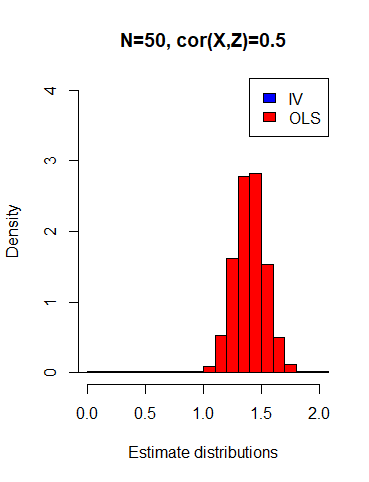
\includegraphics[width=\linewidth]{Fig1.png}
    \end{minipage}
    \begin{minipage}[b]{0.5\linewidth}
        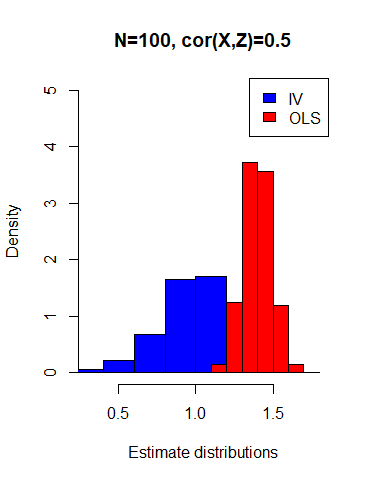
\includegraphics[width=\linewidth]{Fig2.png}
    \end{minipage}
    \begin{minipage}[b]{0.5\linewidth}
        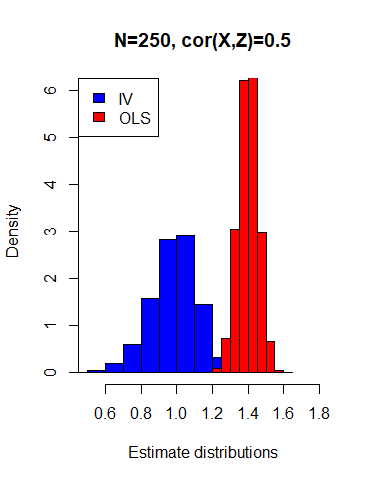
\includegraphics[width=\linewidth]{Fig3.png}
    \end{minipage}
    \begin{minipage}[b]{0.5\linewidth}
        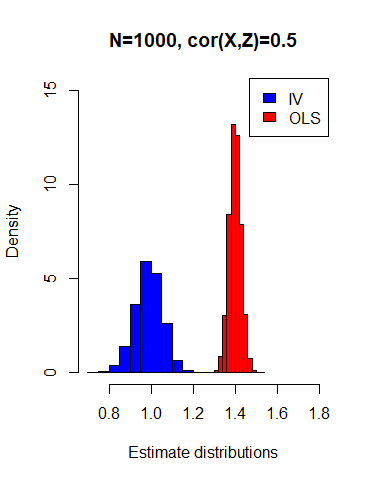
\includegraphics[width=\linewidth]{Fig4.png}
    \end{minipage}\hfill
    \label{Cor50}
    \caption{Distributions of IV and OLS estimates when $\rho_{XZ}=0.5$}
\end{figure}

As we can see, as long as the sample size increases we see that the distribution variance decreases both for the OLS and IV estimator. This is the graphic representation of the consistency property. Moreover, we can see graphically also the demonstration of the efficiency property of the OLS. OLS indeed shows a consistent lower variance and the frequency of the median values rises faster. In other words, IV estimator distribution is flatter than the OLS one. However, it is evident that OLS distribution is biased, contrary to the IV. Indeed, while the IV estimator distribution is centered on 1, the OLS distribution is centered around 1.4. The bias is positive and is exactly equal to $\cfrac{Cov(x,\epsilon)}{\sigma^2_x}$. Since $Cov(x,\epsilon)=\rho_{x\epsilon}\sigma_x$, the bias is equal to $\cfrac{\rho_{x\epsilon}}{\sigma_x}\approx 0.4$. From these graphs, then it is clear that, in a non-biased setting the IV estimates may have more problems with the statistical inference. The IV errors are indeed larger than the OLS.

\subsection{b) Weaker instruments:}
\textbf{Now repeat the analysis from a), but instead assume that the correlation between the instrument $z$ and the regressor $x$ is $0.15$. Discuss the difference in sampling distributions between OLS and IV and, in addition, discuss the difference between sampling distributions based on weak and strong IVs.}

\begin{figure}[p!]
    \begin{minipage}[b]{0.5\linewidth}
        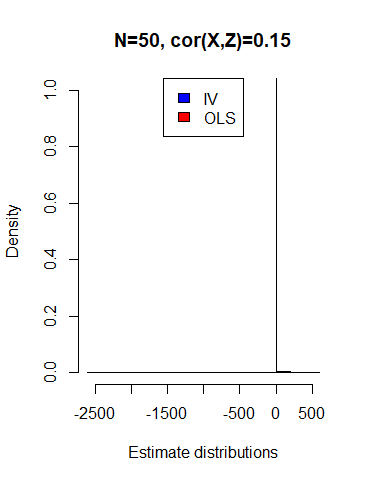
\includegraphics[width=\linewidth]{Fig1A.png}
    \end{minipage}
    \begin{minipage}[b]{0.5\linewidth}
        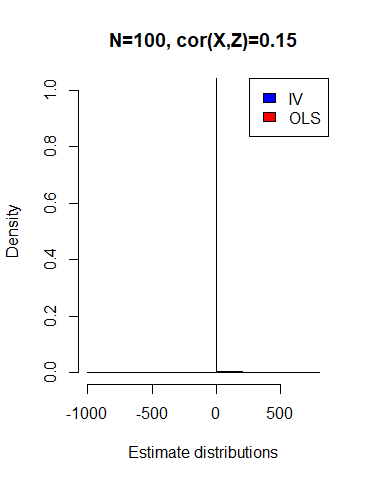
\includegraphics[width=\linewidth]{Fig2A.png}
    \end{minipage}
    \begin{minipage}[b]{0.5\linewidth}
        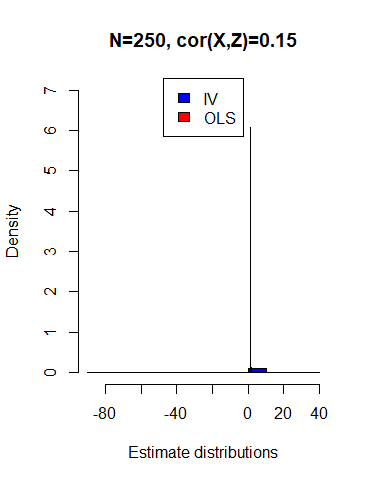
\includegraphics[width=\linewidth]{Fig3A.png}
    \end{minipage}
    \begin{minipage}[b]{0.5\linewidth}
        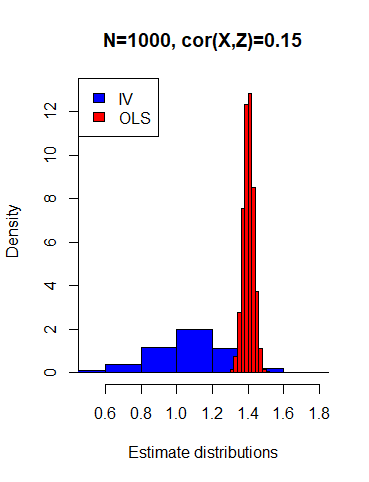
\includegraphics[width=\linewidth]{Fig4A.png}
    \end{minipage}\hfill
    \label{cor15}
    \caption{Distributions of IV and OLS estimates when $\rho_{XZ}=0.15$}
\end{figure}

In figure \ref{cor15} we can hardly observe the OLS distribution for a problem of scale, however it remains basically unchanged. In the IV case, we can notice a very different scenario. The IV distribution is much flatter than the previous case. To fully grasp the difference we can observe the scale of the axes. While in figure \ref{Cor50}, the top-right graph presents an interval between 0.3 and 1.7, in figure \ref{cor15} the same graph the interval is between -1000 and 600. This is due to the formula of the variance for the IV estimator. The asymptotic variance of the IV is:
\[
\widehat{Avar}(\beta^{IV}-\beta|X,Z)=E[(Z'X)^{-1}Z'uu'Z(Z'X)^{-1}|X,Z]
\]
\[
\widehat{Avar}(\beta^{IV}-\beta)=E[uu'](Z'X)^{-1}=\Sigma^2_u(Z'X)^{-1}
\]
The asymptotic variance of the IV estimator can be written as the variance matrix of the error times the inverse of the covariance of Z and X. In our simple univariate case $Z'X=Cov(x,z)=\rho_{xz}\sigma_z\sigma_x$=. The variance of the estimator, then, is inversely related to $\rho_{xz}$. For this reason, the weaker is the instrument and the higher is the variance of the IV estimator. This leads to problems for the statistical inference since the results are not significant even if unbiased.

\newpage
\section{3. Empirical Application}

The empirical application is based on a cross-sectional dataset assign2.dta, which contains the following variables:
\begin{itemize}
    \item \textit{age}: age of surveyed individual
    \item \textit{logearn}: log annual earnings
    \item \textit{yob}: year of birth
    \item \textit{schooling}: age at which the person left school.
\end{itemize}

a) The goal is to estimate the returns to education. For this purpose, we estimate an OLS regression of \textit{logearn} on schooling, controlling for fourth-order polynomials in age and year of birth. Interpret the coefficient of schooling.

The model that we estimate with the 4th order polynomial is given as:
\begin{multline}
    logearn_i = \beta_0 + \beta_1 {schooling} + \beta_2 {age} + \beta_3 {age^2} + \beta_4 {age^3} + \beta_5 {age^4} \\
    + \beta_6 {yob} + \beta_7 {yob^2} + \beta_8 {yob^3} + \beta_9 {yob^4} + \epsilon_i
\end{multline}

\begin{table}[!htbp] \centering 
  \caption{Regression Summary: OLS with controlling for 4th order polynomial for age and yob} 
  \label{reg 1} 
\begin{tabular}{@{\extracolsep{5pt}}lc} 
\\[-1.8ex]\hline 
\hline \\[-1.8ex] 
 & \multicolumn{1}{c}{\textit{Dependent variable:}} \\ 
\cline{2-2} 
\\[-1.8ex] & logearn \\ 
\hline \\[-1.8ex] 
 schooling & 0.158$^{***}$ \\ 
  & (0.002) \\ 
  & \\ 
 age & $-$0.254 \\ 
  & (0.540) \\ 
  & \\ 
 age\_sq & 0.009 \\ 
  & (0.017) \\ 
  & \\ 
 age\_cube & $-$0.0001 \\ 
  & (0.0002) \\ 
  & \\ 
 age\_4 & 0.00000 \\ 
  & (0.00000) \\ 
  & \\ 
 yob & 0.441$^{*}$ \\ 
  & (0.252) \\ 
  & \\ 
 yob\_sq & $-$0.018 \\ 
  & (0.012) \\ 
  & \\ 
 yob\_cube & 0.0003 \\ 
  & (0.0002) \\ 
  & \\ 
 yob\_4 & $-$0.00000 \\ 
  & (0.00000) \\ 
  & \\ 
 Constant & 1.489 \\ 
  & (6.176) \\ 
  & \\ 
\hline \\[-1.8ex] 
Observations & 30,801 \\ 
R$^{2}$ & 0.147 \\ 
Adjusted R$^{2}$ & 0.147 \\ 
Residual Std. Error & 0.494 (df = 30791) \\ 
F Statistic & 591.542$^{***}$ (df = 9; 30791) \\ 
\hline 
\hline \\[-1.8ex] 
\textit{Note:}  & \multicolumn{1}{r}{$^{*}$p$<$0.1; $^{**}$p$<$0.05; $^{***}$p$<$0.01} \\ Values in the parentheses are the standard errors.\\The dependent variable is logged earnings.
\end{tabular} 
\end{table}

In table \ref{reg 1} , we present the regression summary of the simple OLS model while controlling for the fourth order polynomials of age and year of birth. In the table, we see that the estimate for schooling is significant at 1\%. Where as the estimate for year of birth is also significant at 10\%. We see that with an additional year of schooling $\beta = 15.8$\% causing $15.8\%$ increase in earnings. This is only true when we control for higher order polynomials in our regression. In order for us to not to over-fit or under-fit the model we use the higher order polynomial. Additionally, despite adding the higher order polynomials we see the estimated $R^2$ and the $Adjusted R^2$ is 14.7\%\\

An additional step carried out is to compare the model from table \ref{reg 1} to table \ref{reg 2}. As we can see the results in the table \ref{reg 2}
are the summary findings when we do not have higher order polynomials. We simply estimate the logged earnings as a function of age , year of birth (yob) and schooling. In this particular regression, we see that all the variables are significant at 90\%. Additionally, the estimate for schooling is 15.7 indicating that there is rise in earnings by 15.7\% with an additional year of schooling. This estimate is in particular very close to the estimate obtained in table \ref{reg 1}. The adjusted $R^2$ and the $R^2$ in this case is comparatively smaller at 14\%. Therefore, we can conclude by saying that using the higher order polynomials is a better fit.\\


\begin{table}[!htbp] \centering 
  \caption{Regression Summary: A Simple OLS Model} 
  \label{reg 2} 
\begin{tabular}{@{\extracolsep{5pt}}lc} 
\\[-1.8ex]\hline 
\hline \\[-1.8ex] 
 & \multicolumn{1}{c}{\textit{Dependent variable:}} \\ 
\cline{2-2} 
\\[-1.8ex] & logearn \\ 
\hline \\[-1.8ex] 
 age & 0.005$^{***}$ \\ 
  & (0.001) \\ 
  & \\ 
 yob & 0.005$^{***}$ \\ 
  & (0.001) \\ 
  & \\ 
 schooling & 0.157$^{***}$ \\ 
  & (0.002) \\ 
  & \\ 
 Constant & 2.964$^{***}$ \\ 
  & (0.055) \\ 
  & \\ 
\hline \\[-1.8ex] 
Observations & 30,801 \\ 
R$^{2}$ & 0.140 \\ 
Adjusted R$^{2}$ & 0.140 \\ 
Residual Std. Error & 0.496 (df = 30797) \\ 
F Statistic & 1,673.896$^{***}$ (df = 3; 30797) \\ 
\hline 
\hline \\[-1.8ex] 
\textit{Note:}  & \multicolumn{1}{r}{$^{*}$p$<$0.1; $^{**}$p$<$0.05; $^{***}$p$<$0.01} \\ The vales in the parentheses are standard errors\\(This regression is additional \\and used to compare regression with 4th order polynomial)
\end{tabular} 
\end{table} 

\textbf{A common way to obtain causal estimates is to use changes in compulsory schooling laws for identification. In this case, birth cohorts born before 1933 $(yob<33)$ had to go to school until they were 14 years old, whereas compulsory schooling age was raised to 15 years for all cohorts born from 1933 onwards. This change in compulsory schooling laws can be used as an instrumental variable for the actual duration of schooling. The instrument is a dummy LAW that equals unity if a person is born 1933 or later and zero otherwise.} \\

\textbf{b) Discuss this instrument in theory, assuming that schooling $S_i$ is related to the instrument $Z_i$ by the latent assignment mechanism
\begin{equation*}
    S_i = 1(\gamma_0+ \gamma_1 Z_i > \eta_i),\;\; with\;\; E(Z_i \eta _i) = 0
\end{equation*}
The random variable $\eta_i$ represents the individual resistance to treatment. Why could there be a
first stage? Under what condition is this instrument valid? What are potential threats to validity?
Furthermore, explain who are the compliers, always-takers and never-takers in this case. Would the IV estimate correspond to the average treatment effect (why or why not)?}\\

\textbf{b.1) Instrument Discussion.} The compulsory schooling law indicates the minimum exiting age of education. Provided a similar compulsory law for school entering age which requires students’ enrolment at the same given age, the changes in compulsory schooling law render the actual minimum years of schooling for individuals.

The outcome of the change in law is limited to only affect the exiting age. Strictly speaking, the total year of schooling is only expected to have an increase without definitive entering age of schooling. In other words, the actual duration of schooling may not necessarily change. On the other hand, the law has no impact on any other aspects of education except the duration, for instance, no change in enrolment criteria, tuition fee, teaching quality, evaluation standard and qualification.

The law executes on the basis of birth date which is considered as completely random assignment across individuals. The date of birth is also considered as an independent information that is unlikely associated with the difference in innate ability, or motivation, or family socio-economic background, that would introduce variations in the academic performance, or skill formation, which further leads to various occupations and discrepancy in income. Thus, we agree that all the other demographic factors are uncorrelated to the date of birth, and no reverse impact of date of birth. Then, based on the year of birth, the instrument is as good as randomly assigned.

Given the latent assignment mechanism equation, \(\gamma_0+ \gamma_1 Z_i > \eta_i\), by construct, the instrument triggers the behavioural change through the preference threshold that defined by the resistance to treatment. There are three components in the equation: first, the fixed initial state of preference over resistance to treatment, $\gamma_0$; second, the span of alteration in preference corresponds to the individual response to the instrument, where the magnitude difference for the binary alteration in preference is captured by the parameter of willingness to accept the new law, $\gamma_1$; third, the fixed threshold of individual resistance to treatment, $\eta_i$. Thus, the channel of variation only presents in the second component.

Assumption, \( E(Z_i \eta _i) = 0\), states that the resistance is independent of instrument. The resistance then must originate from other individual level characteristics, such as perspective of usefulness of schooling, direct cost of enrolment and opportunity cost of foregone earnings, which are uncorrelated to the new schooling law. On the other hand, the consideration of having compulsory additional year of schooling has no interest to affect the resistance. The law only activates this particular acceptance of new regulation in addition to the initial state which exceeds the resistance threshold to have individuals selected into the treatment. 

This mechanism equation then further characterises the heterogeneity in compliant sub-population.  Groups of complier, never-taker, always-taker, and defier, which are indicated by the values of each parameter and the signs of $\gamma_1$. For instance, always-taker has initially high $\gamma_0$ to be treated without the presence of second term; never-taker may have high $\eta_i$, or small $\gamma_1$, or small $\gamma_0$ that impossible to exceed as the resistance threshold; defier typically has the negative sign for $\gamma_1$.\\

\textbf{b.2) First Stage.} 
There could be a first stage if 
\begin{align}
  S_i =S_{0i}+(S_{1i}-S_{0i})Z_i &=\alpha_0 + \alpha_1 Z_i + \xi_i \\
E(S_{0i}-S_{1i}) &= 0  
\end{align}
From the assignment equation \(\gamma_0+ \gamma_1 Z_i > \eta_i\), we have the heterogeneous $\gamma_0$, $\gamma_1$, and the $\eta_i$. Such variations at individual level suggest that the behavioural change of having older graduation age cannot be completely determined by the instrument. Thus, ${S_i}$ is a function of heterogeneous response to the instrument, where $S_{0i}$ and $S_{1i}$ have different mean, $Z_i$ has effect on $S_i$. Suppose we have heterogeneous individuals $\emph{i} \not= $\emph{j},
\begin{align*}
  \alpha_{0i} & \not= \alpha_{0j} \\
  \alpha_{1i} & \not= \alpha_{1j} \\
  \eta_i & \not= \eta_j \\
\end{align*}
\textbf{b.3) Instrument Validity.}
Except first stage, there are three assumptions need to hold for the validity of instrument.

\textbf{Independence Assumption.} The instrument is based on birth year, and the date of birth is considered completely random and independent of individual decision. When the instrument design is independent of demographic structure, i.e., the treatment assignment criteria is independent of subjective decision on socio-economic background, we may agree that the instrument assignment is therefore satisfies independence assumption.

\textbf{Exclusion Restriction.} Given our outcome variable of interest is individual growth in earnings, the birth year is unlikely correlated with the innate ability, motivation, interest of profession, which are observable and will affect the earnings, i.e. $E(Z|\epsilon_i)=0$, where the earnings by design are assumed to vary only because of the change in duration of compulsory schooling.

\textbf{Monotonicity.} The instrument aims to introduce one additional year of schooling. When the instrument at least not reducing the actual minimum duration of schooling, the monotonicity assumption is satisfied. Given the change in duration is based on the previous compulsory schooling law, individuals are expected to at least not affected if they previously complied to the law. In other words, monotonicity holds as long as the instrument is independent of individual resistance to treatment.\\

\textbf{b.4) Potential Threats.} From the internal validity by design, individuals may not receive the treatment which increase the duration of schooling. Consider the actual years of schooling is determined by both age of entering and age of exiting, the current compulsory schooling law only fixes one side of the duration. Although without any intuitive reason, there is possibility that individuals are treated but would still have the same duration (may even decrease) of schooling due to late enrolment (older entering age) and gap year (interrupted schooling). Thus, the design does not guarantee homogeneous treatment effect, instead, we may observe a heterogeneous treatment effect across population. Together with the uncertainty of policy implementation, the heterogeneous treatment effect weakens the instrument, which leads to nonzero correlation between instrument and treatment. This weak first-stage correlation will increase the variance that leads to estimation inconsistency and unreliable inference.

In addition, at the time of observation, later the birth year less the working experience. We argue that income may grow at different rate for different age, where seniors tend to have higher income but little growth. Now depart from the differences among age groups, the reduced form estimate omits the effect of growing up environment for the cohorts, where cohort born at the same year are likely to share certain background which is different from other years. Regarding the demographic structure, birth year is not as good random as date of birth at days or months. The birthday cut off is “more” random compared to the completion of academic year. That says, there is difference for cohorts who born before and who born after the instrument, then the instrument is not assigned randomly, the independence assumption may be violated.

For external validity at different contexts, additional information (such as tuition fee, other direct education cost, opportunity cost of foregone earning, subject taught, skill acquisition, labour market, etc.) are likely to violate the exclusion restriction and independence assumption. For instance, the affordability of the additional year of schooling may negatively associated with the individual resistance to treatment, thus the instrument will correlate with the unobserved confounding characteristics of not being treated and even positively associated with factors that lead to little income growth. When consider the upper tail of high in \emph{$logearn_i$}, duration of minimum schooling may not be informative, particularly for those who later obtained higher education. Similarly for the lower tail, the identification valid only when we impose strong assumption that individual always invest more on education within their constraints whenever it is possible. Thus, the extrapolating the LATE requires additional information from the population as well as reasonable assumptions on them. \\

\textbf{b.5) Compliant Subpopulation.} The compliant subpopulation is characterised by the construct of assignment mechanism, where the three components vary at individual level. And by assumption, the compliant type exclusively depends on the resistance that originates from the individual background.

Since from complier, $D_0_i=1$ and $D_1_i=1$, regardless which behavioural component that assigns individual into treatment, the resistance to treatment is overcome. For complier, the resistance must greater than the initial state ($\gamma_0$ < $\eta_i$), which means without the presence of new law, complier would not opt in for the duration of schooling.

For always-taker, $D_0_i=D_1_i=1$, we have ($\gamma_0$ > $\eta_i$), which means the resistance to treatment on this instrument is always less than the initial state. With or without the law, always-taker would have longer duration of schooling, they are unaffected by the instrument given potentially high motivation to invest in education. For never-taker, $D_0_i=D_1_i=0$, they also will be unaffected by the presence of instrument given ($\gamma_0$ + $\gamma_1$$Z_i$ < $\eta_i$) where the resistance is sufficiently large enough to prevent any behavioural change.  \\

\textbf{b.5) LATE and ATE.} 
The causal effect of treatment on the treated includes both ATE on complier and always-taker, which is different from the IV estimate that only captures the ATE on complier. Similar argument holds for ATE of treatment on untreated.

Suppose that how the instrument will affect the individual to be assigned to be treatment is not determined by composition of population, provided a constant treatment effect of ATT, the larger the complier size, the greater the LATE. Thus, IV estimate corresponds to the ATE. Now consider an alternative population where the composition of compliance differs, LATE decrease as the share of complier shrinks, where the IV gives the LATE for compliers, ATE is reduced in magnitude.

Then, the unconditional ATE is the weight average of effects on all compliant subpopulation, and by monotonicity where the never-taker and always-taker are differenced out, the IV estimate obtained from Wald estimator essentially corresponds to the magnitude of ATE as well as the composition of sub-population.

\newpage

\textbf{c) As in any good empirical project, begin with a graphical inspection of the relationships of interest. This is best done through binscatters. Produce and discuss the graphs listed below. In all graphs, include a vertical line at $yob=33$.}\\

\begin{itemize}
    \item \textbf{Plot the probability that a person leaves school before age 15 against the year of birth.}
\end{itemize}
 {\begin{figure}[h!]
    \centering
    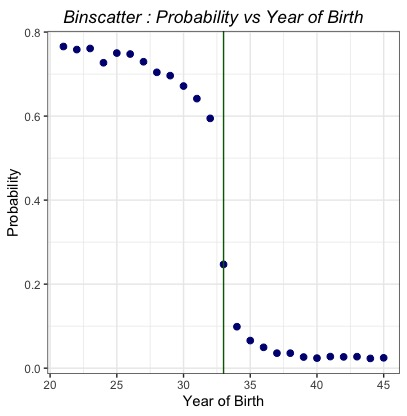
\includegraphics[width=0.6\textwidth]{Binscatter 2.jpeg}
    \caption{Binscatter - Probability of a person leaving school before 15 years of schooling}
    \label{fig 1}
    \end{figure}}
The figure \ref{fig 1} is the binscatter of the Probability of an individual leaving school before the age of 15 plotted against the year of birth. We the see the green line vertically at the year of birth 1933. This line indicates the instrument that is the law of compulsory schooling till 15 years of age. As we can see, the probability of leaving school before 15 years is close to 0.8 before the law and has fallen drastically after the law. We find this to be an interesting observation.\\
\begin{itemize}
    \item \textbf{Binscatter of schooling and year of birth}
\end{itemize}

     {\begin{figure}[h!]
    \centering
    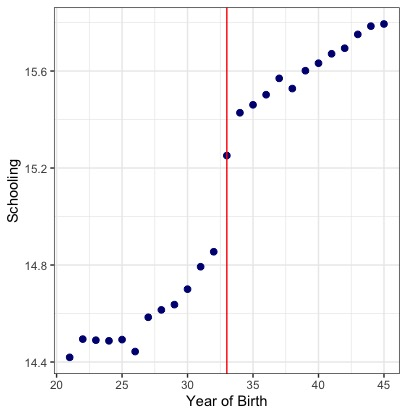
\includegraphics[width=0.6\textwidth]{Binscatter 1.jpeg}
    \caption{Binscatter - Schooling and year of birth}
    \label{fig 2}
    \end{figure}}
In figure \ref{fig 2}, we present the binscatter of Schooling in years with the year of birth. We also include the vertical line in red indicating the year of birth $=33$. We believe that including this line gives us clear idea of what happened post implementation of the law of compulsory schooling which was implemented in 1933. We see that, most of the observations after this mark, have a steadily rising years of schooling. In conclusion, people who were given the instrument, particularly the compliers have seen undergone the treatment.
\\
\begin{itemize}
    \item \textbf{Binscatter of log earnings and year of birth.}
\end{itemize}
      {\begin{figure}[h!]
    \centering
    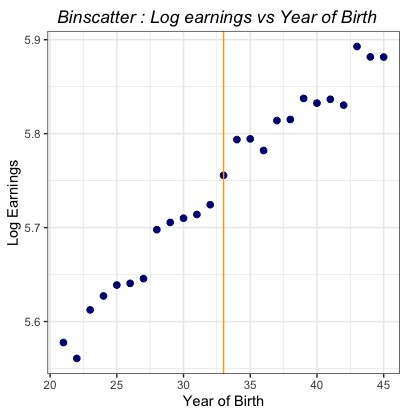
\includegraphics[width=0.6\textwidth]{Binscatter 3.jpeg}
    \caption{Binscatter - Logged Earnings and year of birth}
    \label{fig 3}
    \end{figure}}

Finally, in figure \ref{fig 3}, we see the binscatter of Logged Earnings and year of birth. This figure helps us understand if the treatment was significant in improving the earnings of individuals. With the oragne line indicating the year of birth as 1933, the year of compulsory 15 years of schooling law. We see that earnings have risen up-to 58\% with additional schooling years. In conclusion, we can say that, the law (in the case of compilers) have witnessed a significant increase because of undergoing the treatment which in this case is schooling.

\newpage
\textbf{d) Calculate the Wald estimator (without controls) "by hand", i.e. based on conditional averages. Compare your results to those of a 2SLS estimation based on an inbuilt command (e.g. \textit{ivregress} in Stata or \textit{ivreg} in R). Interpret your results and compare them to the OLS results in a)}\\

Table \ref{reg 3} summarises the regression results for instrument variable (\textit{LAW}) and outcome variable (\textit{logearn}). With the presence of instrument, i.e., the LAW, duration of schooling increased by 0.99 unit, at 1\% statistically significance level, which is approximately one additional year. Based on the first stage results, we agree that the law of compulsory schooling until 15 years old is a valid instrument. In addition, consider the expected effect of instrument on schooling year is one additional year, which is unit of 1, the first stage estimate with value of 0.990 implies a considerable share of complier and always-taker. In fact, the intercept term with value of 14.634 also implies that without the presence of instrument, the sample mean of schooling exiting age is almost 15 years old. Consider the compliers will be only enrolled until 14 years old, followed by the discussion in previous section, value of 14.634 for constant term may suggest a dominant proportion of complier who will only enrol in school until 14 years old, $E(D_c|Z_0)=14$. Thus, suppose the number of always-taker is also small, We may expect a similar coefficient estimate from the Wald estimator as compared to reduced form results. \\ 

From the reduced form, presented in table \ref{reg 4} is the estimate of the outcome on the instrument is given as 0.162. To obtain the Wald Estimator manually we simply obtain the ratio of: 
\\
\begin{align*}
       \cfrac{ITT(Reduced Form)}{The first stage}
\end{align*}
 

\begin{center}
    0.162/0.990 = 0.1633267 
\end{center}
\\
\begin{table}[!htbp] \centering 
  \caption{Regression Summary : Treatment and Instrument} 
  \label{reg 3} 
\begin{tabular}{@{\extracolsep{5pt}}lc} 
\\[-1.8ex]\hline 
\hline \\[-1.8ex] 
 & \multicolumn{1}{c}{\textit{Dependent variable:}} \\ 
\cline{2-2} 
\\[-1.8ex] & schooling \\ 
\hline \\[-1.8ex] 
 LAW & 0.990$^{***}$ \\ 
  & (0.014) \\ 
  & \\ 
 Constant & 14.624$^{***}$ \\ 
  & (0.012) \\ 
  & \\ 
\hline \\[-1.8ex] 
Observations & 30,801 \\ 
R$^{2}$ & 0.137 \\ 
Adjusted R$^{2}$ & 0.136 \\ 
Residual Std. Error & 1.146 (df = 30799) \\ 
F Statistic & 4,868.939$^{***}$ (df = 1; 30799) \\ 
\hline 
\hline \\[-1.8ex] 
\textit{Note:}  & \multicolumn{1}{r}{$^{*}$p$<$0.1; $^{**}$p$<$0.05; $^{***}$p$<$0.01} \\ The values in parenthesis are standard errors.
\end{tabular} 
\end{table} 

\\

In table \ref{reg 4} we present a formal discussion of the results of imposing the law of compulsory schooling up-to 15 years and returns to education , i.e, instrument and outcome. As we can see, the estimate obtained is 0.162, indicating that upon the imposition of the law, earnings are likely to increase by 16.2\% provided an individual complies with the law and under goes the treatment. And this causality occurs via schooling. We call this the reduced form or intention to treat (ITT).\\

\begin{table}[!htbp] \centering 
  \caption{Regression Summary: Outcome and Instrument} 
  \label{reg 4} 
\begin{tabular}{@{\extracolsep{5pt}}lc} 
\\[-1.8ex]\hline 
\hline \\[-1.8ex] 
 & \multicolumn{1}{c}{\textit{Dependent variable:}} \\ 
\cline{2-2} 
\\[-1.8ex] & logearn \\ 
\hline \\[-1.8ex] 
 LAW & 0.162$^{***}$ \\ 
  & (0.007) \\ 
  & \\ 
 Constant & 5.671$^{***}$ \\ 
  & (0.005) \\ 
  & \\ 
\hline \\[-1.8ex] 
Observations & 30,801 \\ 
R$^{2}$ & 0.019 \\ 
Adjusted R$^{2}$ & 0.019 \\ 
Residual Std. Error & 0.530 (df = 30799) \\ 
F Statistic & 607.678$^{***}$ (df = 1; 30799) \\ 
\hline 
\hline \\[-1.8ex] 
\textit{Note:}  & \multicolumn{1}{r}{$^{*}$p$<$0.1; $^{**}$p$<$0.05; $^{***}$p$<$0.01} \\ The values in parentheses are standard errors.
\end{tabular} 
\end{table} 
\\
The findings from using the "ivreg" command in R, are summarised in table \ref{reg 5} .To establish a casual estimate we regress earnings on the treatment. As we can see, the estimate for schooling is 0.1633, the estimate is also significant at 1\%. The estimate same as the Wald estimator calculated manually. The adjusted $R^2$ is at 13.8\% indicating that schooling causes 13.8\% variation in the earnings with an additional year of schooling. Additionally, this is caused by the instrument, compulsory schooling upto 15 years of age. 
\\
\begin{table}[!htbp] \centering 
  \caption{IVREG with R code} 
  \label{reg 5} 
\begin{tabular}{@{\extracolsep{5pt}}lc} 
\\[-1.8ex]\hline 
\hline \\[-1.8ex] 
 & \multicolumn{1}{c}{\textit{Dependent variable:}} \\ 
\cline{2-2} 
\\[-1.8ex] & logearn \\ 
\hline \\[-1.8ex] 
 schooling & 0.163$^{***}$ \\ 
  & (0.006) \\ 
  & \\ 
 Constant & 3.283$^{***}$ \\ 
  & (0.095) \\ 
  & \\ 
\hline \\[-1.8ex] 
Observations & 30,801 \\ 
R$^{2}$ & 0.138 \\ 
Adjusted R$^{2}$ & 0.138 \\ 
Residual Std. Error & 0.497 (df = 30799) \\ 
\hline 
\hline \\[-1.8ex] 
\textit{Note:}  & \multicolumn{1}{r}{$^{*}$p$<$0.1; $^{**}$p$<$0.05; $^{***}$p$<$0.01} \\ The values in parenthesis are standard errors.
\end{tabular} 
\end{table} 


\end{document}
